\section{Parsing}
{\tiny analyzing a string of symbols to discover its (inherent) structure
}\\
\scriptsize{Top-down parsing} 
{\tiny Start from S, find a sequence of derivations that yield the sentence\\
predict: generate a hypothesis based on the grammar\\
match: when a terminal symbol is produced, check if it matches with the one in the expected position(if matched, continue; otherwise, backtrack)\\
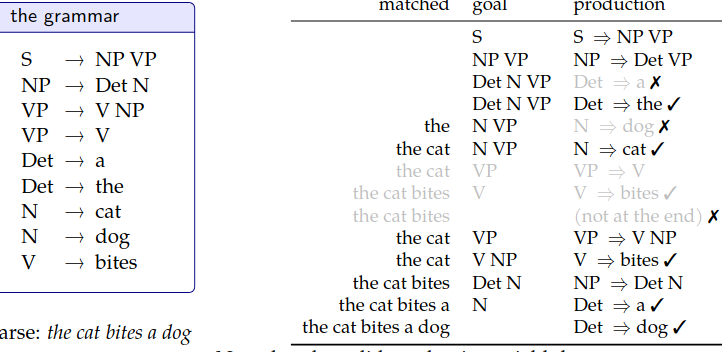
\includegraphics[scale=0.2]{top-down.png}\\
trial-and-error procedure leads to exponential time parsing; some rules may cause infinite loops
}\\
\scriptsize{Bottom-up parsing}\\ {\tiny Start from from the input symbols, and try to reduce the input to start symbol\\
shift-reduce: \\
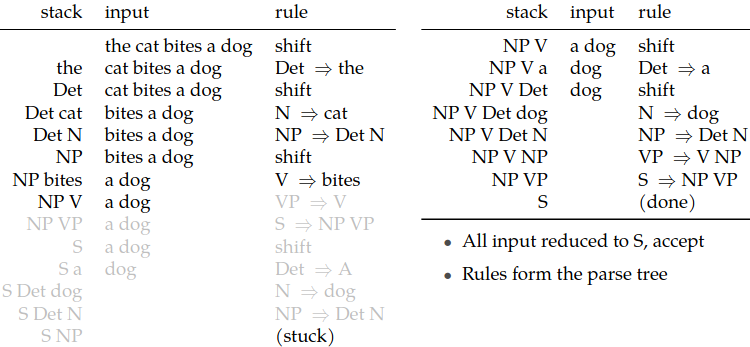
\includegraphics[scale=0.2]{shift-reduce.png}
}
\subsection*{CKY algorithm}
{\tiny a dynamic programming algorithm; processes the input bottom up, and saves the intermediate results on a chart\\ 
time complexity O(n**3); space complexity O(n**2)\\
requires the CFG to be in Chomsky normal form (CNF)
}\\
\scriptsize{Chomsky normal form(CNF)}\\ {\tiny A->B C, A->a, where A,B,C are non-terminals and a is a terminal\\
converting to CNF: \\
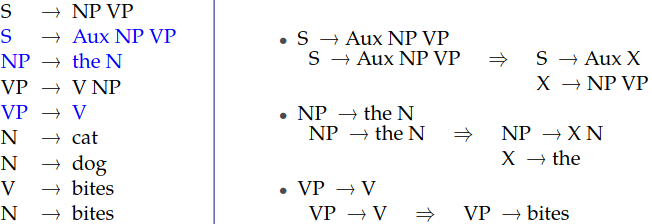
\includegraphics[scale=0.2]{convertion-cnf.png}\\
}\\
\scriptsize{CKY demo}
{\tiny 
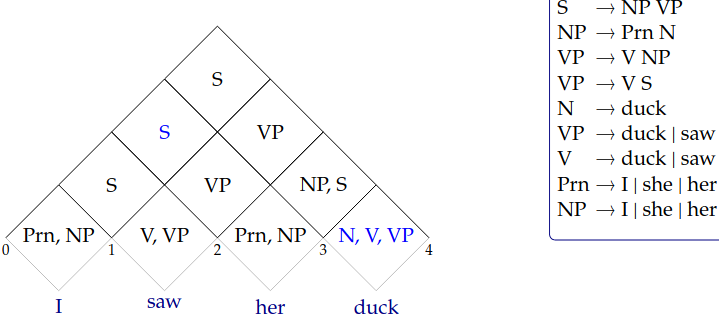
\includegraphics[scale=0.2]{cky-demo.png}\\
to recover parse trees, we follow the same procedure as recognition, add back links to keep track of the derivations\\
avoids re-computing the analyses by storing the earlier analyses (of sub-spans) in a table\\
efficiently stores a parse forest\\
enumerating all possible parses have exponential complexity (worst case)
}\\
\subsection*{Earley algorithm}
{\tiny a top down (and left-to-right) parsing algorithm\\
keep records of constituents that are predicted, in-progress and completed at every position in the input string\\
time complexity O(n**3), space complexity O(n**2)\\
the Earley chart stores a parse forest compactly, but extracting all trees may require exponential time\\
can process any CFG (no need for CNF)
}\\
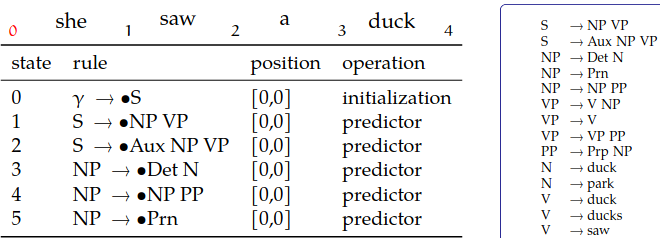
\includegraphics[scale=0.2]{earley0.png}\\
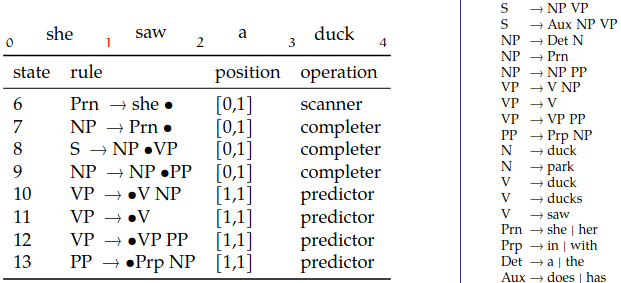
\includegraphics[scale=0.2]{earley1.png}\\
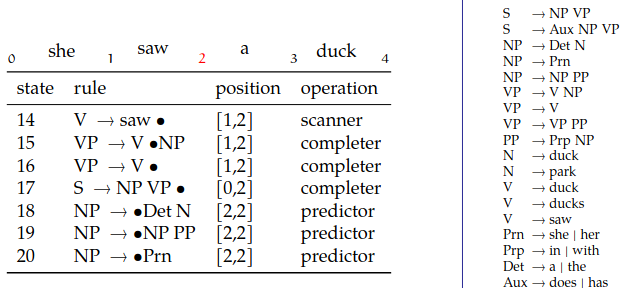
\includegraphics[scale=0.2]{earley2.png}\\
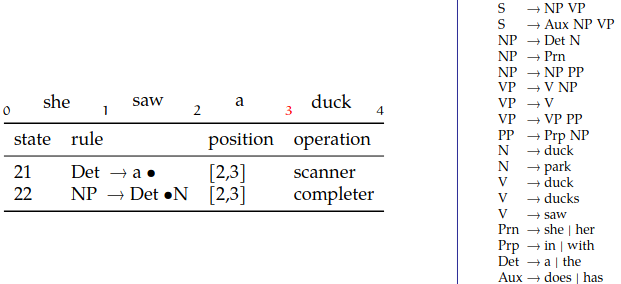
\includegraphics[scale=0.2]{earley3.png}\\
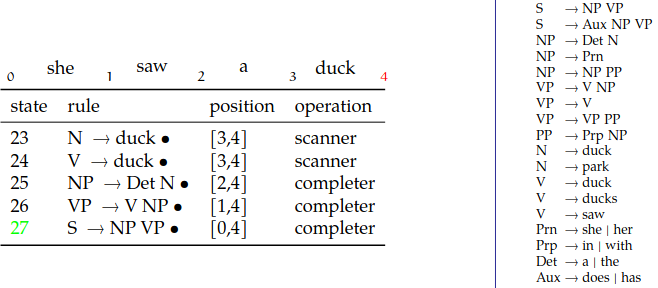
\includegraphics[scale=0.2]{earley4.png}
\subsection*{Dependency parsing}
\scriptsize{Grammar-driven}\\
\scriptsize{Data-driven}\\ {\tiny The ‘grammar’, and the (soft) constraints are learned from a treebank\\
Graph-based: search for the best tree structure, e.g. find minimum spanning tree, adaptations of CF chart parser(e.g. CKY)\\
Transition-based: similar to shit-reduce parsing, single pass over the sentence, determine an operation(shift or reduce) at each step; linear time complexity; need an approximate method to determine the best operation
}\\
\scriptsize{Transition-based parsing} {\tiny
Linear time, greedy, projective parsing\\
Can be extended to non-projective dependencies\\
need some extra work for generating gold-standard transition sequences from treebanks\\
Early errors propagate, transition-based parsers make more mistakes on long-distance dependencies\\
The greedy algorithm can be extended to beam search for better accuracy (still linear time complexity)\\
the shift-reduce (LR) parsers for formal languages are deterministic, actions are determined by a table lookup\\
Natural language sentences are ambiguous, a dependency parser’s actions cannot be made deterministic\\
Operations are (somewhat) different: instead of reduce (using phrase-structure rules) we use arc operations connecting two words with a labeled arc\\
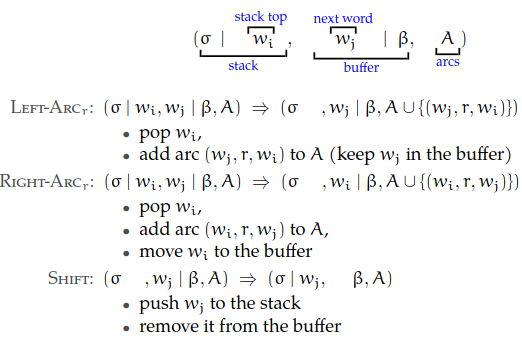
\includegraphics[scale=0.2]{transition-system.png}\\
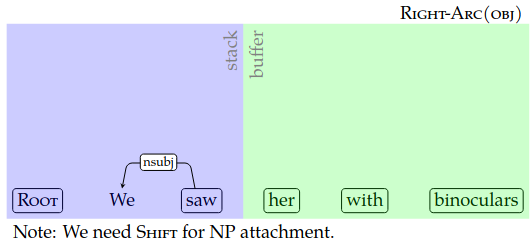
\includegraphics[scale=0.2]{transition-system1.png}\\
}\\